\section{Introduction}
\begin{frame}
	\frametitle{Introduction}
	We can derive the mathematical model of a dynamic system in \textbf{two ways} mainly:
	\begin{enumerate}
		\item Physical Modeling: 
		
		Applying the laws of physics, chemistry, thermodynamics,...
		Also called modeling from \emph{First Principles}
		
		\begin{itemize}
			\item Sometimes these are non-linear. Lots of methods of this course require linear systems. Therefore \textbf{linearization} is  needed.
			
			\hspace{1cm} e.g. $\sin(\theta) \sim \theta, \theta \rightarrow 0$
		\end{itemize}
		\pause 
		
		\item  System identification or \emph{Empirical Modeling}:
		
		Developing models from observed or collected data
		
	\end{enumerate}
	
\end{frame}

\begin{frame}
	\frametitle{Main classes of System identification methods}
	\textbf{White box modeling}: based on first principles. \\
	$\rightarrow$ known equations (structure) $\&$ parameters (coefficients). \\
	\ \newline
	\pause
	\textbf{Grey box identification}: first principles $\&$ experimentation. \\
	$\rightarrow$ known equations, unknown/uncertain parameters. \\
	\ \newline
	\pause
	\textbf{Black box identification}: based on experimentation. \\
	$\rightarrow$ unknown equations $\&$ unknown parameters. \\
	\ \newline
	\pause
	Most popular approaches are forms of black box identification.
\end{frame}


\section{First Principles Modeling}

% Counter for the example numbers
\newcounter{exampleCount}

\begin{frame}
	\stepcounter{exampleCount}
	\frametitle{Example \arabic{exampleCount}: Mass-Spring System} 
	
	\begin{columns}
		\begin{column}{0.4\linewidth}
			\begin{figure}
				\centering
				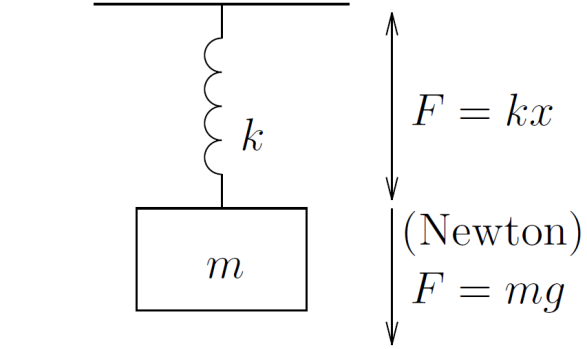
\includegraphics[width=1\linewidth]{img/mass-spring}
				\label{fig:mass-spring}
			\end{figure}
		\end{column}
		\begin{column}{0.6\linewidth}
			If spring is at rest at $x=0$:
			\begin{align*}
			m \cdot \frac{d^{2}x}{dt^{2}} + k \cdot x =  m \cdot g \\
			\end{align*}
		\end{column}
	\end{columns}
\end{frame}


\begin{frame}
	\stepcounter{exampleCount}
	\frametitle{Example \arabic{exampleCount}: Mass-Spring Damped}
	\begin{figure}
		\centering
		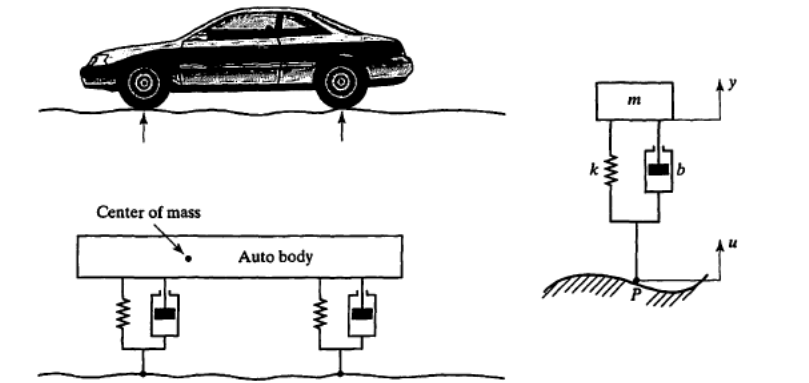
\includegraphics[width=1\linewidth]{img/mass-spring-damped}
		\label{fig:mass-spring-damped}
	\end{figure}
	Force exerted by damper: $F = b\dot{x}$
	
	Differential equation can be found by writing force equilibrium and moment equilibrium around center of mass
	
	%\emph{\textcolor{blue}{ \href{https://youtu.be/8DuJEpy-ODo}{Animation} }}
\end{frame}

\begin{frame}
	\stepcounter{exampleCount}
	\frametitle{Example \arabic{exampleCount}: Pendulum}
	\begin{columns}
		\begin{column}{0.4\linewidth}
			\begin{figure}
				\centering
				\includegraphics[width=1\linewidth]{img/new-pendulum}
				\label{fig:pendulum}
			\end{figure}
		\end{column}
		\begin{column}{0.6\linewidth}
			Dynamic equilibrium:
			\begin{align*}
			&I\ddot{\theta}(t) = -m g \frac{L}{2} \sin(\theta(t)) \text{ with } I= \frac{m L^2}{3} \\
			&\ddot{\theta}(t)  = -\frac{3g}{2L} \sin(\theta(t)) 
			\end{align*}
			
			Small deviation of $\theta(t)$: \\
			\hspace{1cm} $\ddot{\theta}(t) = -\frac{3g}{2L} \theta(t)$
			
			Solving the differential equation yields the general solution:
			$\theta(t) = A\cos(\omega_0 + \phi)$
			with $\omega_0=\sqrt{\frac{3g}{2L}}$ and $\phi$ \& $A$ to be determined with the initial condition
		\end{column}
	\end{columns}
\end{frame}

\begin{frame}
	\stepcounter{exampleCount}
	\frametitle{Example \arabic{exampleCount}: Inverted Pendulum}
	\begin{columns}
		\begin{column}{0.6\linewidth}
			\begin{figure}
				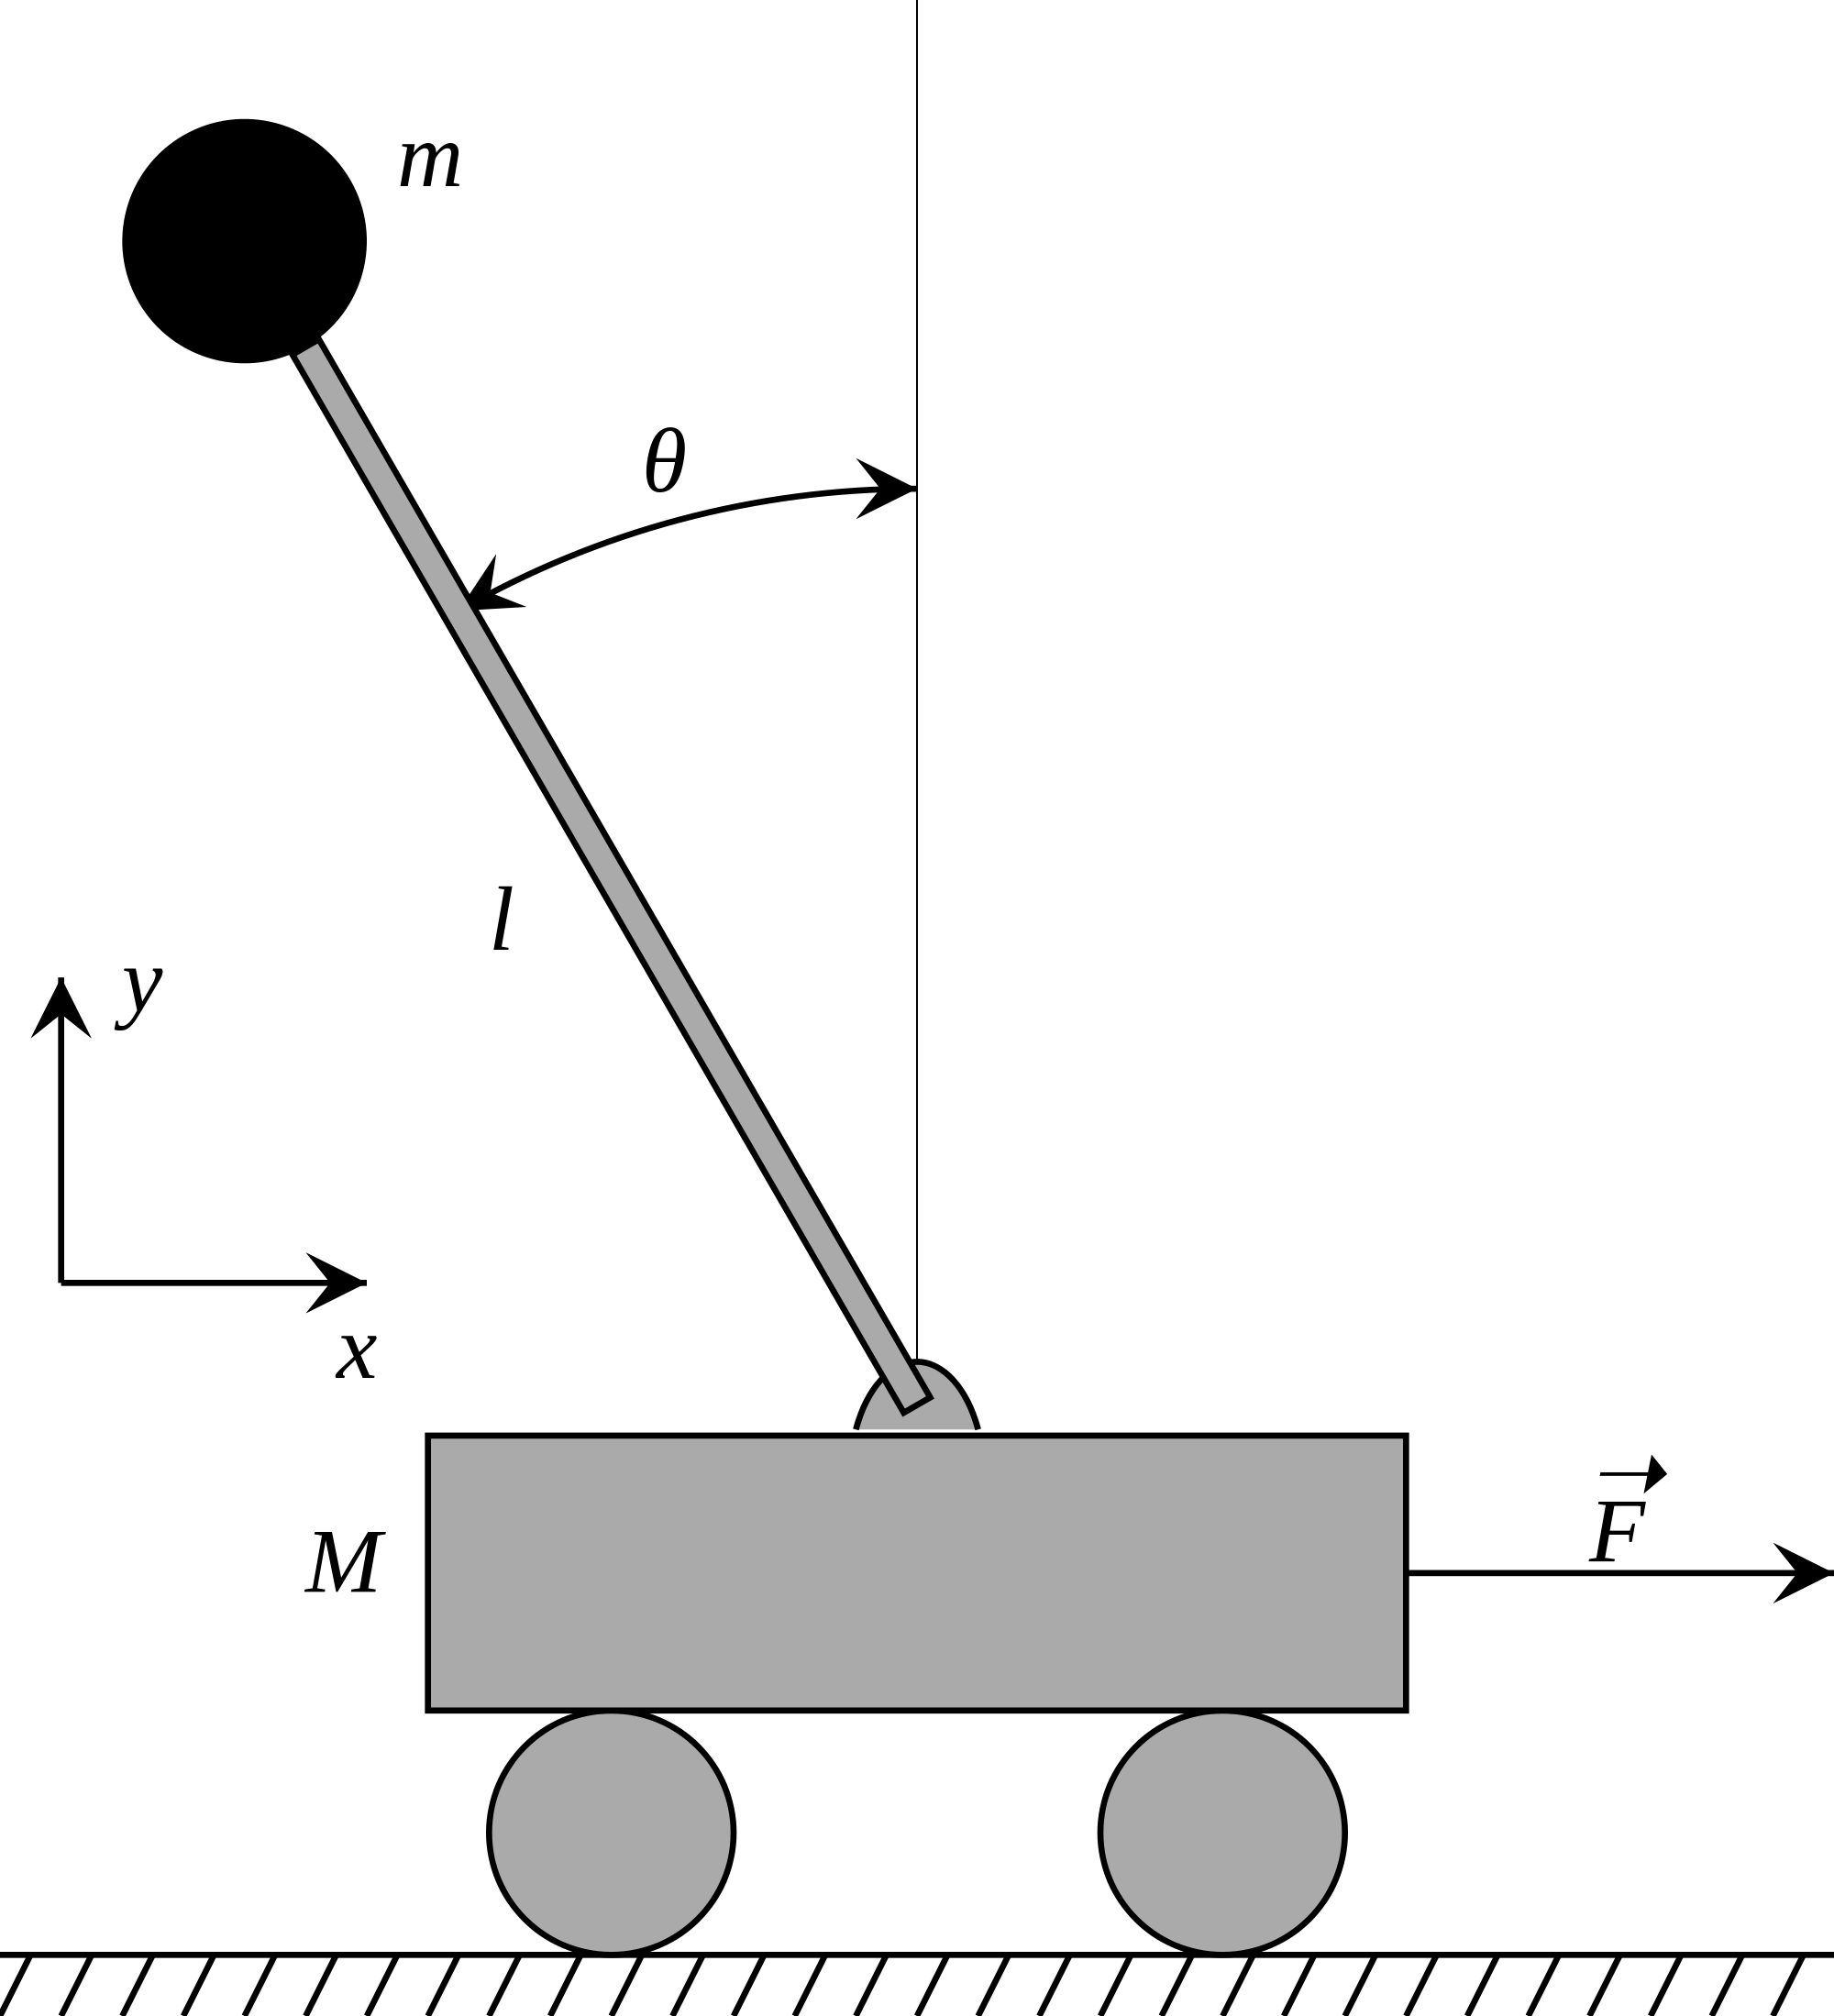
\includegraphics[width=0.9\linewidth]{img/pendulum-inverted}
				\label{fig:pendulum-inverted}
				%youtube: https://www.youtube.com/watch?v=15DIidigArA
			\end{figure}
		\end{column}
		\begin{column}{0.4\linewidth}
			Analysis can be done with Newton like former example, but less tedious is using energy-methods (Lagrange)
			
		\end{column}
	\end{columns}
	
\end{frame}

\begin{frame}
	\stepcounter{exampleCount}
	\frametitle{Example \arabic{exampleCount}: RLC Circuit}
	
	\begin{figure}
		\centering
		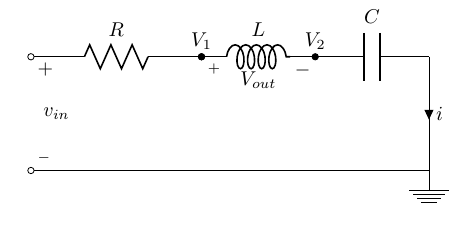
\includegraphics[width=0.7\linewidth]{img/circuit-RLC}
		\label{fig:circuit-RLC}
	\end{figure}
	Besides input $v_{in}$, two internal variables are needed to determine output $\Rightarrow$ Second-order System
	\begin{center}
		\begin{tabular}{c@{\hskip 1cm} c@{\hskip 1cm} c}
			Inputs 	& Ouputs 	& Choosen States \\ \hline
			$v_{in}$ 	& $v_{out}$	& $V_2$ \\
			& & $i$ \\ 
		\end{tabular}
	\end{center}
	
\end{frame}

\begin{frame}
	
	\frametitle{Example \arabic{exampleCount}: RLC Circuit}
	
	\begin{columns}
		\begin{column}{0.4\linewidth}
			Equations for each component:
			\begin{align*}
				&i = \frac{V_{in} - V_{1}}{R} 		&\text{\small(Ohm's law)}\\
				&V_1 - V_2 = L \cdot \frac{di}{dt} 	&\text{\small(Coil)}\\
				&i = C \cdot \frac{dV_2}{dt} 	 	&\text{\small(Capacitor)}
			\end{align*}
		\end{column}
		\begin{column}{0.6\linewidth}
			\begin{figure}
				\centering
				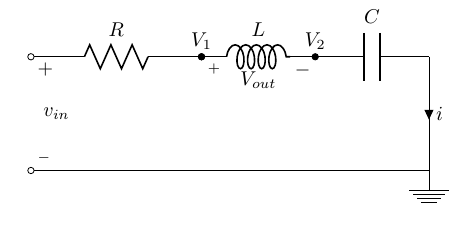
\includegraphics[width=1\linewidth]{img/circuit-RLC}
				\label{fig:circuit-RLC-small}
			\end{figure}
		\end{column}
		
	\end{columns}
	
\end{frame}

\begin{frame}
	
	\frametitle{Example \arabic{exampleCount}: RLC Circuit}
	\begin{itemize}
		\item Writing derivatives of state variables in function of state variables and inputs: 
		$ \left\lbrace  \begin{matrix}
		\frac{di}{dt} = \frac{V_1 - V_2}{L} = \frac{V_{in} - R\cdot i - V_2}{L} \\
		\frac{dV_2}{dt} 
		= \frac{i}{C}	\\
		\end{matrix} 
		\right. 
		$
		\item Writing output in function of state variables and inputs: $V_{out} = V_1 - V_2 = V_{in} - Ri - V_2$
	\end{itemize}
	\begin{block}{State Space Representation}
		This yields the \textbf{State Space Representation} of the dynamic system. In Matrix form:
		\begin{align*}
		\begin{bmatrix}
		\frac{dV_2}{dt} \\
		\frac{di}{dt} \\
		\end{bmatrix} 
		&= 
		\begin{bmatrix}
		0 & 1/C \\
		-1/L & -R/L  \\
		\end{bmatrix} 	
		\begin{bmatrix}
		V_2 \\
		i \\
		\end{bmatrix}
		+ 
		\begin{bmatrix}
		0 \\
		1 \\
		\end{bmatrix}
		V_{in} 
		\\
		V_{out} &= 
		\begin{bmatrix}
		-1 & -R
		\end{bmatrix}
		\begin{bmatrix}
		V_2 \\
		i \\
		\end{bmatrix}
		+ V_{in}
		\end{align*}
	\end{block}	
\end{frame}

\begin{frame}
	\frametitle{Force-Voltage Analogy}
	
	\begin{figure}
		\centering
		\includegraphics[width=0.9\linewidth]{"img/force-voltage"}
		\label{fig:force-voltageanalogy}
	\end{figure}
	
	
	Let:
	\begin{center}
		\begin{tabular*}{0.4\linewidth}{@{\extracolsep{\fill} }c  c @{$\leftrightarrow$} c }
			F	&&	V \\
			$\dot{x}$ && i \\
			x && q \\
		\end{tabular*}
	\end{center}
	
\end{frame}

\begin{frame}
	\frametitle{Force-Voltage Analogy}
	The analogy between the other quantities follows from comparing the physical laws.
	\vspace{2pt}
	\begin{tabular*}{1\linewidth}{@{\extracolsep{\fill}} l l l }
		Damping: & Resistance: & \\
	\end{tabular*}
	\begin{columns}
		\begin{column}{0.25\linewidth}
			\begin{figure}
				\includegraphics[width=1\linewidth]{img/damping}
			\end{figure}
		\end{column}
		
		\begin{column}{0.25\linewidth}
			\hspace{3pt}
			$F = b\dot{x} $ 
		\end{column}
		
		\begin{column}{0.25\linewidth}
			\begin{figure}
				\centering
				\includegraphics[width=1\linewidth]{img/resistor}
				\label{fig:resistor}
			\end{figure}
		\end{column}
		
		\begin{column}{0.25\linewidth}
			\hspace{3pt}
			$V = Ri$
		\end{column}
		
	\end{columns}
	
	\begin{center}
		$\boxed{b \leftrightarrow R} $	
	\end{center}
\end{frame}

\begin{frame}
	\frametitle{Force-Voltage Analogy}
	\begin{columns}
		\begin{column}{0.25\linewidth}
			Spring:
			\begin{figure}
				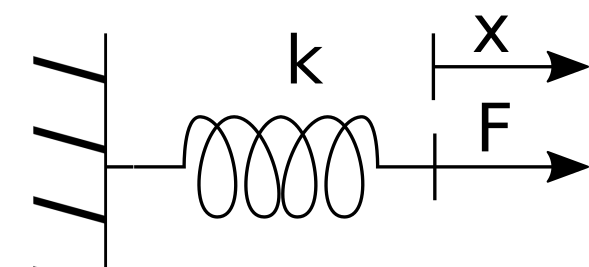
\includegraphics[width=1\linewidth]{img/spring}
			\end{figure}
		\end{column}
		
		\begin{column}{0.25\linewidth}
			\hspace{3pt}
			$F = kx \newline \Rightarrow \frac{dF}{dt} = k\frac{dx}{dt}$ 
		\end{column}
		
		\begin{column}{0.25\linewidth}
			Capacitor:
			\begin{figure}
				\includegraphics[width=1\linewidth]{img/capacitor}
				\label{fig:capacitor}
			\end{figure}
		\end{column}
		
		\begin{column}{0.25\linewidth}
			\hspace{3pt}
			$\frac{dV}{dt} = \frac{i}{C}$
		\end{column}
		
	\end{columns}
	
	\begin{center}
		$\boxed{k \leftrightarrow \frac{1}{C}} $	
	\end{center}
	
	\pause
	
	\begin{columns}
		\begin{column}{0.25\linewidth}
			Newton:
			\begin{figure}
				\includegraphics[width=1\linewidth]{img/newton}
			\end{figure}
		\end{column}
		
		\begin{column}{0.25\linewidth}
			\hspace{3pt}
			\begin{align*}
			F &= m \ddot{x} \\ 
			&= m \frac{d\dot{x}}{dt}
			\end{align*} 
		\end{column}
		
		\begin{column}{0.25\linewidth}
			Coil:
			\begin{figure}
				\includegraphics[width=1\linewidth]{img/coil}
				\label{fig:coil}
			\end{figure}
		\end{column}
		
		\begin{column}{0.25\linewidth}
			\hspace{3pt}
			$V = L\frac{di}{dt}$
		\end{column}
		
	\end{columns}
	
	\begin{center}
		$\boxed{m \leftrightarrow L} $	
	\end{center}
\end{frame}

\begin{frame}
	\stepcounter{exampleCount}
	\frametitle{Example \arabic{exampleCount}: Hoover dam}
	\begin{columns}
		\begin{column}{0.6\linewidth}
			Define:
			\begin{itemize}
				\item Inflow of water: $u(t)$
				\item Current volume of water: $x(t)$
				\item Outflow of water: $y(t)$
				\item Water level: $h(t)$
			\end{itemize}
			Assume that $x(t) = c_1\cdot h(t)$
			
			\vspace{6pt}
			What will happen when we open the gate?
		\end{column}
		\begin{column}{0.4\linewidth}
			\begin{figure}
				\centering
				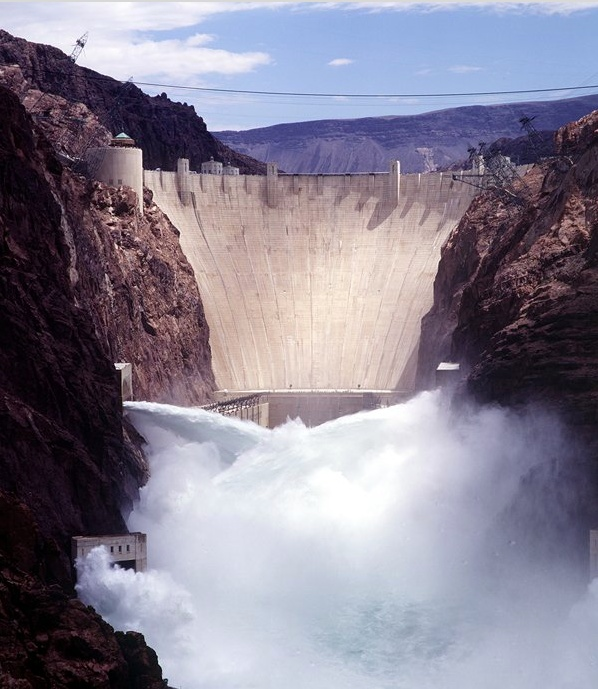
\includegraphics[width=1\linewidth]{img/Hoover-dam}
				\label{fig:Hoover-dam}
			\end{figure}
		\end{column}
	\end{columns}
	
\end{frame}

\begin{frame}
	\frametitle{Example \arabic{exampleCount}: Hoover dam}
	\begin{itemize}
		\item Outflow depends on height: \\
		\hspace{1cm}$y(t) = c_2 \cdot h(t) $
		\item The state of the system is defined by the contained volume of water: \\
		\hspace{1cm}$\dot{x}(t) = u(t) - y(t) = u(t) - c_2\cdot h(t) $
		\item Thus a \textbf{State Space Representation} is, with $c \triangleq \frac{c_2}{c_1}$:
		\begin{align*}
		\dot{x}(t) &= u(t) - c\cdot x(t) \\
		y(t) &= c\cdot x(t) \\
		\end{align*} 
	\end{itemize}
	\vspace{-1cm}
	\begin{center}
		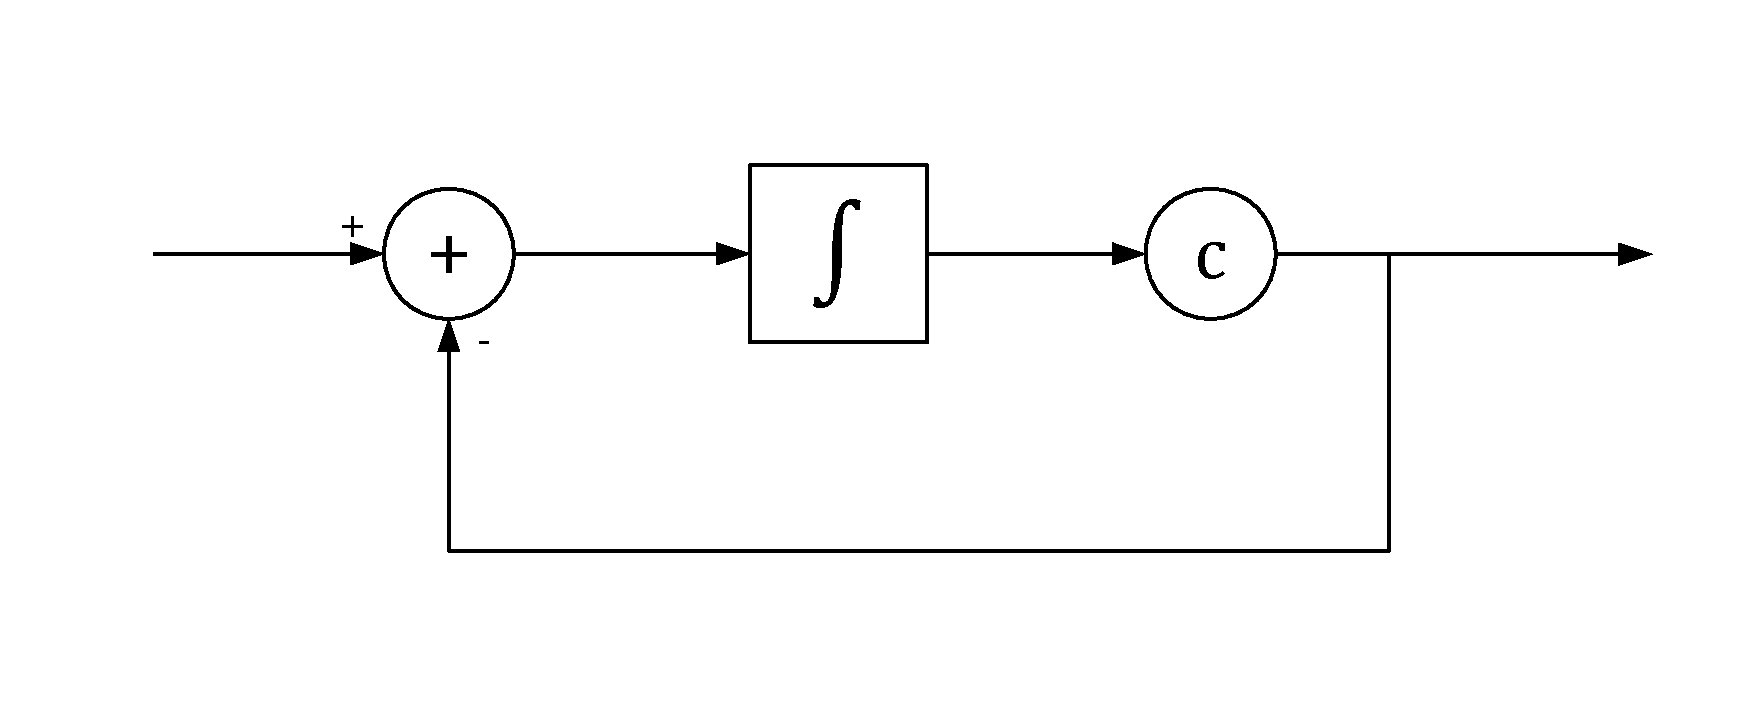
\includegraphics[width=0.75\linewidth]{img/hoover-dam-diagram}
	\end{center}
\end{frame}

\section{Nonlinear systems \& linearization}
\begin{frame}
	\frametitle{Nonlinear systems}
	In this course we focus on the linear state-space representation:
	\begin{align*}
	\left\{ \begin{matrix} 
	\dot{x}(t) = A x(t) + B u(t), \\ 
	y(t) = C x(t) + D u(t).
	\end{matrix}\right.\quad\quad
	\left\{ \begin{matrix} 
	x[k+1] &= A x[k] + B u[k], \\ 
	y[k] &= C x[k] + D u[k].
	\end{matrix}\right.
	\end{align*}
	\pause
	\ \newline
	Most real life systems involve nonlinearity:
	\begin{align*}
	\left\{ \begin{matrix} 
	\dot{x}(t) = f\big(x(t), u(t)\big), \\ 
	y(t) = g\big(x(t), u(t)\big),
	\end{matrix}\right.
	\end{align*}
	where $f$ and/or $g$ contain some nonlinearity, such as:
	\begin{itemize}
		\item \emph{powers}: e.g. $\dot{x}(t) = A x(t) + B u(t) {\color{blue}+ \gamma u(t)^2}$,
		\item \emph{interactions}: e.g. $\dot{x}(t) = A x(t) + B u(t) {\color{blue}+ \gamma x(t) u(t)}$,
		\item \emph{clipping}: e.g. ${\color{blue}\alpha \leq }x(t){\color{blue}\leq \beta}$.
	\end{itemize}
\end{frame}

\begin{frame}
	\frametitle{Linearization around equilibrium point}
	Nonlinear systems have (several) equilibrium points $x_e$, $u_e$, $y_e$:
	\begin{align*}
	\left\{ \begin{matrix}
	\dot{x}_e = f\big(x_e, u_e\big)=0, \hfill \\
	y_e = g\big(x_e, u_e\big). \hfill
	\end{matrix}\right.
	\end{align*}
	\pause
	Linearizing in the region of $(x_e, u_e, y_e)$:
	\begin{align*}
	x = x_e + \Delta x, \quad u = u_e + \Delta u, \quad y = y_e + \Delta y,
	\end{align*}
	with $\Delta x$, $\Delta u$ and $\Delta y$ \emph{sufficiently} small.\\
	\ \newline
	\pause
	Linearizing is done via \textbf{first order Taylor expansions}.
\end{frame}

\begin{frame}
	\frametitle{Linearization around equilibrium points}
	Linearizing is done via \textbf{first order Taylor expansions}.
	\begin{align*}
	\left\{ \begin{matrix}
	\frac{dx}{dt} = \frac{d (x_e + \Delta x)}{dt} = \frac{d \Delta x}{dt} = f(x,u) = f(x_e+\Delta x, u_e + \Delta u), \\
	y_e + \Delta y = g(x, u) = g(x_e + \Delta x, u_e + \Delta u).
	\end{matrix}\right.
	\end{align*}
	We write the \emph{vectors} $x$ and $u$ in their individual components to simplify interpretation:
	\begin{align*}
		\dot{x}_1 &= f_1(x_1, ..., x_n, u_1, .., u_l) \\
			&\vdots \\
		\dot{x}_n &= f_1(x_1, ..., x_n, u_1, .., u_l) \\
		\dot{y}_1 &= h_1(x_1, ..., x_n, u_1, .., u_l) \\
			&\vdots \\
		\dot{y}_l &= h_l(x_1, ..., x_n, u_1, .., u_l) 
	\end{align*}
\end{frame}

\begin{frame}
	\frametitle{Linearization around equilibrium points}
	The first order Taylor expansion of $f()$ around $(x_e,u_e)$ is described by the \textbf{Jacobian Matrix}:
	\begin{align*}
		\dfrac{dx}{dt} = f(x_e,u_e) +
					\begin{bmatrix}
						\dfrac{\partial f_1}{\partial x_1} 	&\dots 	&\dfrac{\partial f_1}{\partial x_n} 	&\dfrac{\partial f_1}{\partial u_1} 	&\dots 	&\dfrac{\partial f_1}{\partial u_l} \\
						\vdots 						&		&							&					&		&\vdots  \\
						\dfrac{\partial f_n}{\partial x_1} 	&\dots 	&\dfrac{\partial f_n}{\partial x_n} 	&\dfrac{\partial f_n}{\partial u_1} 	&\dots 	&\dfrac{\partial f_n}{\partial u_l} \\
					\end{bmatrix}
					\begin{bmatrix}
						\Delta x_1 \\
						\vdots \\
						\Delta x_n \\
						\Delta u_1 \\
						\vdots \\
						\Delta u_l
					\end{bmatrix}
	\end{align*}
	With the partial derivatives evaluated in $x_e$ and $u_e$
	
	$f(x_e,u_e)=\frac{dx_e}{dt} = 0$ because we \emph{choose} $x_e$ and $u_e$ to be equilibrium points 
\end{frame}

\begin{frame}
	\frametitle{Linearization around equilibrium points}
	This can be split up in a contribution by the state $x$ and the input $u$:
	\begin{align*}
		\dfrac{d\Delta x}{dt} =
		\underbrace{\begin{bmatrix}
						\dfrac{\partial f_1}{\partial x_1} 	&\dots 	&\dfrac{\partial f_1}{\partial x_n} 	\\
						\vdots 								&		&\vdots  								\\
						\dfrac{\partial f_n}{\partial x_1} 	&\dots 	&\dfrac{\partial f_n}{\partial x_n} 	\\
					\end{bmatrix}}_A
		\begin{bmatrix}
			\Delta x_1 \\
			\vdots \\
			\Delta x_n \\
		\end{bmatrix}
		+
		\underbrace{	\begin{bmatrix}
							\dfrac{\partial f_1}{\partial u_1} 	&\dots 	&\dfrac{\partial f_1}{\partial u_l} 	\\
							\vdots 								&		&\vdots 								\\ 
							\dfrac{\partial f_n}{\partial u_1}	&\dots 	&\dfrac{\partial f_n}{\partial u_l}		\\
						\end{bmatrix}}_B
		\begin{bmatrix}
			\Delta u_1 \\
			\vdots \\
			\Delta u_l 
		\end{bmatrix}
	\end{align*}
	Similarly $C$ \& $D$ can be constructed from the Jacobian Matrix of $h(x,u)$
\end{frame}
	


\begin{frame}
	\frametitle{Example: decalcification plant}
	Used to reduce concentration of calcium hydroxide in water:
	\begin{itemize}
		\item chemical reaction: $Ca(OH)_2 + CO_2 \rightarrow CaCO_3 + H_2O$
		\item reaction speed: $r = c[Ca(OH)_2][CO_2]$
		\item rate of change of concentration:
		\begin{align*}
		\frac{d[Ca(OH)_2]}{dt} = \frac{k}{V} - \frac{r}{V}, \\
		\frac{d[CO_2]}{dt} = \frac{u}{V} - \frac{r}{V}, 
		\end{align*}
		with inflow rates $k$ and $u$ in mol/s and tank volume $V$ in L.
		\item input $u$: inflow of $CO_2$, output: $[Ca(OH)_2]$
	\end{itemize}
\end{frame}

\begin{frame}
	\frametitle{Nonlinear model and equilibrium point}
	{\color{red}Nonlinear} model for the given reactor:
	\pause
	\begin{align*}
	\frac{d[Ca(OH)_2]}{dt} &= \frac{k}{V} - \frac{c}{V}{\color{red}[Ca(OH)_2][CO_2]}, \\
	\frac{d[CO_2]}{dt} &= \frac{u}{V} - \frac{c}{V}{\color{red}[Ca(OH)_2][CO_2]}, \\
	y &= [Ca(OH)_2],
	\end{align*}
	with two state variables: ${\color{blue}x_1=[Ca(OH)_2]}$ and ${\color{blue}x_2=[CO_2]}$.\\
	\ \newline
	\pause
	The equilibrium point ${\color{blue}(k_{eq}, u_{eq}, x_{1,eq}, x_{2,eq}, y_{eq})}$ of this system is:
	\pause
	\begin{align*}
	\frac{{\color{blue}k_{eq}}}{V} - \frac{c}{V}{\color{blue}[Ca(OH)_2]_{eq}[CO_2]_{eq}} = 0, \\
	\frac{{\color{blue}u_{eq}}}{V} - \frac{c}{V}{\color{blue}[Ca(OH)_2]_{eq}[CO_2]_{eq}} = 0. \\
	\end{align*}
\end{frame}

\begin{frame}
	\frametitle{Linearization of the decalcification plant}
	For small deviations near the equilibrium:
	\begin{align*}
	\frac{d{\color{blue}\Delta x_1}}{dt} &= -\frac{c}{V} [CO_2]_{eq} {\color{blue}\Delta x_1} - \frac{c}{V} [Ca(OH)_2]_{eq} {\color{blue}\Delta x_2}, \\
	\frac{d{\color{blue}\Delta x_2}}{dt} &= -\frac{c}{V} [CO_2]_{eq} {\color{blue}\Delta x_1} - \frac{c}{V} [Ca(OH)_2]_{eq} {\color{blue}\Delta x_2} + \frac{{\color{blue}\Delta u}}{V}, \\
	{\color{blue}\Delta y} &= {\color{blue}\Delta x_1}.
	\end{align*}
	\pause
	The resulting linear state-space model is $\begin{aligned}\left\{ \begin{matrix} \dot{x}(t) = {\color{green!70!black}A}x(t) + {\color{red}B}u(t) \\ y(t) = Cx(t) + Du(t) \end{matrix}\right.\end{aligned}$:
	\begin{align*}
	\begin{bmatrix}
	\frac{d[Ca(OH)_2]}{dt} \\
	\frac{d[CO_2]}{dt}
	\end{bmatrix} &= 
	{\color{green!70!black}
		-\begin{bmatrix}
		\frac{c}{V}[CO_2]_{eq} & \frac{c}{V}[Ca(OH)_2]_{eq} \\
		\frac{c}{V}[CO_2]_{eq} & \frac{c}{V}[Ca(OH)_2]_{eq} \\
		\end{bmatrix}}
	\begin{bmatrix}
	[Ca(OH)_2] \\
	[CO_2]
	\end{bmatrix} +
	{\color{red}
		\begin{bmatrix}
		0 \\
		\frac{1}{V} \\
		\end{bmatrix}} u(t) \\
	y(t) &= [Ca(OH)_2]
	\end{align*}
\end{frame}

\section{System Identifcation}

\subsection{Grey box identification}
\begin{frame}
	\frametitle{Grey box identification: conceptual}
	Grey box identification starts from a known model structure but with unknown/uncertain parameters $\leftrightarrow$ \textbf{parametric statistics}. \\
	\pause
	\ \newline
	We assume linear, continuous time state space representation:
	\begin{align*}
	\left\{ \begin{matrix} 
	\dot{x}(t) = {\color{blue}A}x(t) + {\color{blue}B}u(t), \\ 
	y(t) = {\color{blue}C}x(t) + {\color{blue}D}u(t).
	\end{matrix}\right.
	\end{align*}
	\pause
	\textbf{Given}: states, inputs, outputs and guesstimates of $\tilde{A}$, $\tilde{B}$, $\tilde{C}$ $\&$ $\tilde{D}$.
	\pause
	\textbf{Task}: estimate $\hat{A}$, $\hat{B}$, $\hat{C}$ and $\hat{D}$ adequately via experiments.\\
	\ \newline
	\pause
	``\emph{All models are wrong, but some are useful.}'' \hfill - George E. P. Box
\end{frame}

\begin{frame}
	\frametitle{Linear regression}
	Consider input matrix $\mathbf{X}$, output vector $\mathbf{y}$ and residuals $\epsilon$:
	\begin{align*}
	\mathbf{X}\theta &= \mathbf{y} + \epsilon.
	\end{align*}
	The parameter vector $\theta$ must be estimated, given the observations.\\
	\pause
	\ \newline
	A common estimation approach is ordinary least squares (OLS):
	\begin{align*}
	(\mathbf{X}^T\mathbf{X})\hat{\theta}_{OLS} &= \mathbf{X}^T\mathbf{y}, \\
	\hat{\theta}_{OLS} &= (\mathbf{X}^T\mathbf{X})^{-1} \mathbf{X}^T\mathbf{y}.
	\end{align*}
	\pause
	The OLS estimate minimizes the sum-of-squares of errors, i.e.:
	\begin{equation*}
	\hat{\theta}_{OLS} = \argmin_{\theta} \sum_{i=1}^N \big(y(i) - \sum_{j=1}^d X(i,j)\theta(j)\big)^2
	\end{equation*}
\end{frame}

\begin{frame}
	\frametitle{Linear regression with ordinary least squares}
	\begin{figure}[!h]
		\centering
		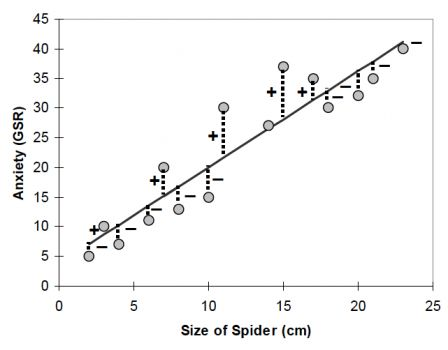
\includegraphics[width=0.8\textwidth]{img/linear-regression.jpg}
	\end{figure}
	\tiny{Image taken from \url{http://freakonometrics.hypotheses.org/2348}}.
\end{frame}


\begin{frame}
	\frametitle{Maximum likelihood estimation}
	The maximum likelihood estimate $\hat{\theta}_{ML}$ is the parameter vector that maximizes the likelihood $\mathcal{L}(\cdot)$ of observing the (known) outputs $\mathbf{y}$, given the (known) inputs $\mathbf{X}$:
	\begin{equation*}
	\hat{\theta}_{ML} = \argmax_{\theta} \mathcal{L}\big(\mathbf{y}, \mathbf{X}\ |\ \theta \big)
	\end{equation*}
	\pause
	For some structures, ML estimate can be obtained in closed form.\\
	\ \newline
	\pause
	\textbf{Example}: least squares estimators are the maximum likelihood estimators if the associated residuals $\epsilon$ are normally distributed.
\end{frame}

\begin{frame}
	\frametitle{Maximum a posteriori (MAP) estimation}
	Bayesian: maximum likelihood estimation with a \emph{prior} $p(\theta)$. \\
	$\rightarrow$ MAP estimation is a regularization of ML estimation \\
	\ \newline
	\pause
	Bayes' theorem: $P(A\ |\ B) = P(B\ |\ A) \cdot P(A)\ /\ P(B)$.\\
	\ \newline
	\pause
	If a prior distribution $p(\cdot)$ is available for $\theta$, then the posterior distribution for $\theta$ becomes:
	\begin{equation*}
	\theta \mapsto \mathcal{L}(\theta\ |\ \mathbf{y}, \mathbf{X}) = \frac{\mathcal{L}(\mathbf{y}, \mathbf{X}\ |\ \theta)p(\theta)}{\int_\vartheta \mathcal{L}(\mathbf{y}, \mathbf{X}\ |\ \vartheta)p(\vartheta)d\vartheta}.
	\end{equation*}
	\pause
	The MAP estimate is the mode of the posterior distribution of $\theta$:
	\begin{equation*}
	\hat{\theta}_{MAP} = \argmax_{\theta} \mathcal{L}(\mathbf{y}, \mathbf{X}\ |\ \theta) p(\theta).
	\end{equation*}
	
\end{frame}

\begin{frame}
	\frametitle{Errors-in-variables approach}
	Additionally accounts for {\color{red}measurement errors in inputs}.\\
	$\leftrightarrow$ standard regression only accounts for {\color{blue}errors in \emph{outputs}} \\
	\ \newline
	\pause
	Typically described via \emph{latent variables}:
	\begin{align*}
	\left\{ \begin{matrix}
	x = x^\star {\color{red}+ \eta}, \\
	y = y^\star {\color{blue}+ \epsilon}, \\
	y^\star = g(x^\star\ |\ \theta),
	\end{matrix}\right.
	\end{align*}
	with $x$, $y$ the observed inputs, outputs and latent variables $x^\star$, $y^\star$.\\
	\pause
	\textbf{Assumption}: latent variables $x^\star$ and $y^\star$ exist which follow the true functional relationship $g(\cdot)$.\\
	\ \newline
	\pause
	\textbf{Task}: estimate $\theta$.
\end{frame}



\subsection{Black box identification}
\begin{frame}
	\frametitle{Black box identification}
	Start from unknown equations $\&$ unknown parameters. \\
	$\rightarrow$ related to \textbf{machine learning} and \textbf{nonparametric statistics}. \\
	\pause
	\ \newline
	If we assume a linear state space system:
	\begin{align*}
	\left\{ \begin{matrix} 
	\dot{x}(t) = A x(t) + B u(t), \\ 
	y(t) = C x(t) + D u(t).
	\end{matrix}\right.\quad\quad
	\left\{ \begin{matrix} 
	x[k+1] &= A x[k] + B u[k], \\ 
	y[k] &= C x[k] + D u[k].
	\end{matrix}\right.
	\end{align*}
	\pause
	\ \newline
	Black box identification deals with:
	\pause
	\begin{itemize}
		\item unknown states, both in number $\&$ physical interpretation \\
		\pause
		$\rightarrow$ dimensions of $A$, $B$ $\&$ $C$ unknown
		\pause
		\item unknown parameters (values in $A$, $B$, $C$, $D$)
	\end{itemize}
\end{frame}

\begin{frame}
	\frametitle{Time series: Santa Fe laser}
	\begin{figure}[!h]
		\centering
		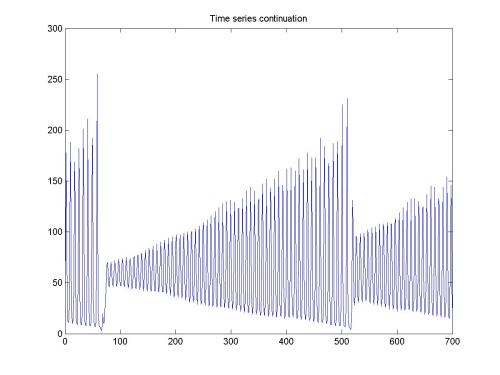
\includegraphics[width=0.8\textwidth]{img/santafe-full.jpg}
	\end{figure}
\end{frame}

\begin{frame}
	\frametitle{Modelling the Santa Fe laster}
	This laser can be treated as an autonomous discrete time system:
	\begin{align*}
	\left\{ \begin{matrix} 
	x[k+1] = f\big(x[k-N+1], \ldots, x[k]\big), \\
	y[k] = x[k]. \hfill
	\end{matrix}\right.
	\end{align*}
	The output depends on the past $N$ states $\&$ no inputs.\\
	\pause
	$\rightarrow$ how large is $N$? $\rightarrow$ \textbf{unknown structure} \\
	\ \newline
	\pause
	Treat it as a regression problem with $N$ inputs: $y = f\big(X_1,\ldots,X_N\big)$. \\
	\pause
	$\rightarrow$ lets say linear, i.e. $y = \mathbf{X}\theta$ $\rightarrow$ \textbf{unknown parameters $\theta \in \mathbb{R}^N$}. \\
	\pause
	$\rightarrow$ for given $N$, we can estimate $\theta$ via grey box methods.\\
	\ \newline
	\pause
	Nonlinear models can be obtained via machine learning methods.
	$\rightarrow$ neural networks, support vector machine, random forest, ...
\end{frame}

\begin{frame}
	\frametitle{Predictions of a least-squares support vector machine}
	\begin{figure}[!h]
		\centering
		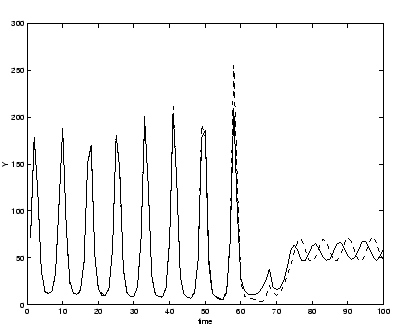
\includegraphics[width=0.8\textwidth]{img/santafe-prediction.png}
	\end{figure}
\end{frame}


\begin{frame}
	\frametitle{Predictions of an artificial neural network}
	\begin{figure}[!h]
		\centering
		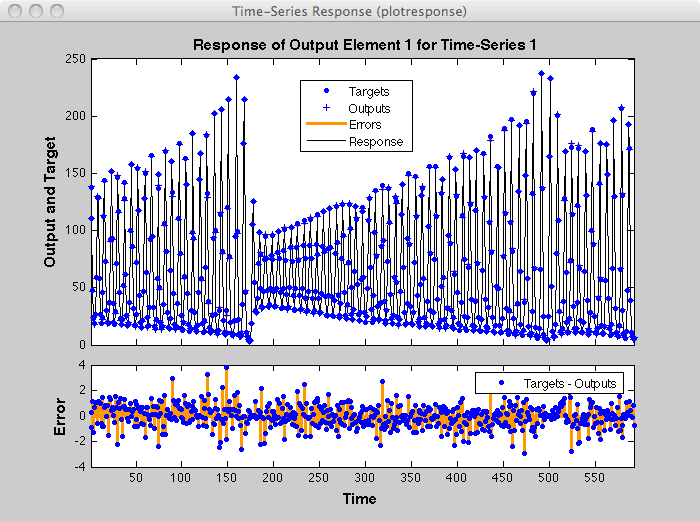
\includegraphics[width=0.8\textwidth]{img/santafe-matlab.png}
	\end{figure}
\end{frame}

\begin{frame}
	\frametitle{Neural network: biological}
	\begin{figure}[!h]
		\centering
		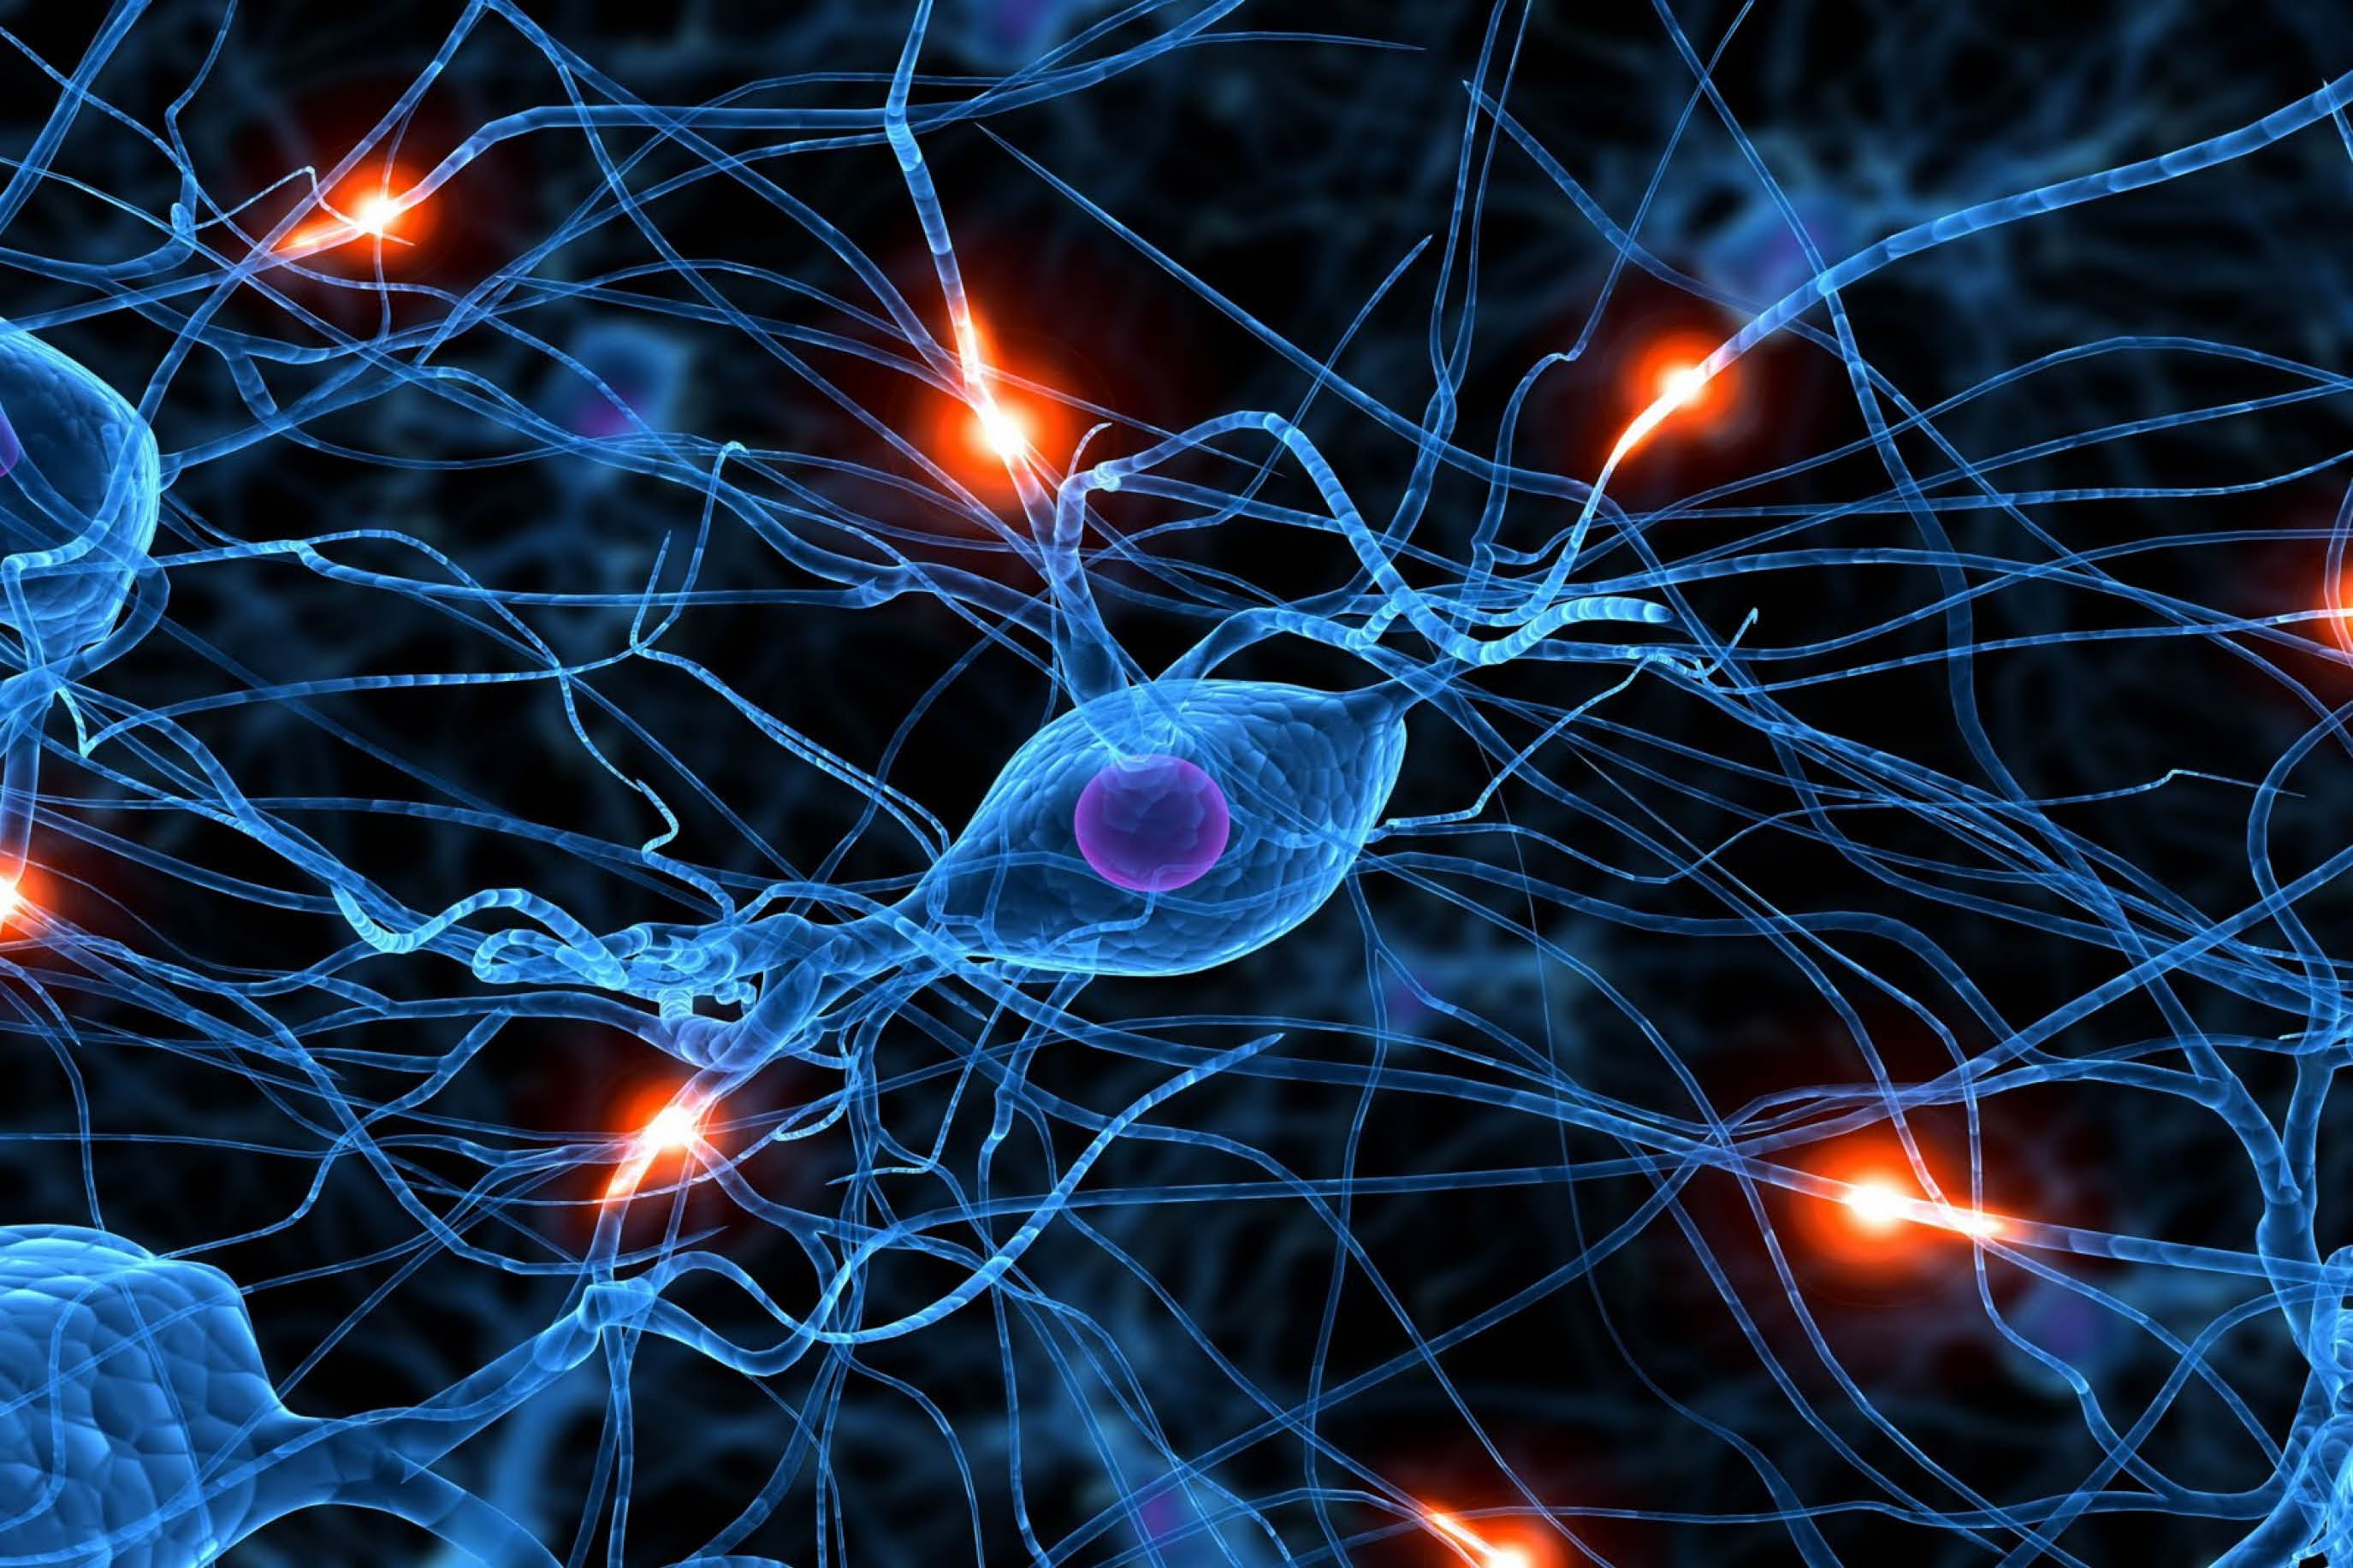
\includegraphics[width=0.9\textwidth]{img/neural-network-cool.jpg}
	\end{figure}
	\tiny{Image taken from \url{http://www.extremetech.com/wp-content/uploads/2013/09/340.jpg}}.
\end{frame}

\begin{frame}
	\frametitle{Structure of a single neuron}
	\begin{figure}[!h]
		\centering
		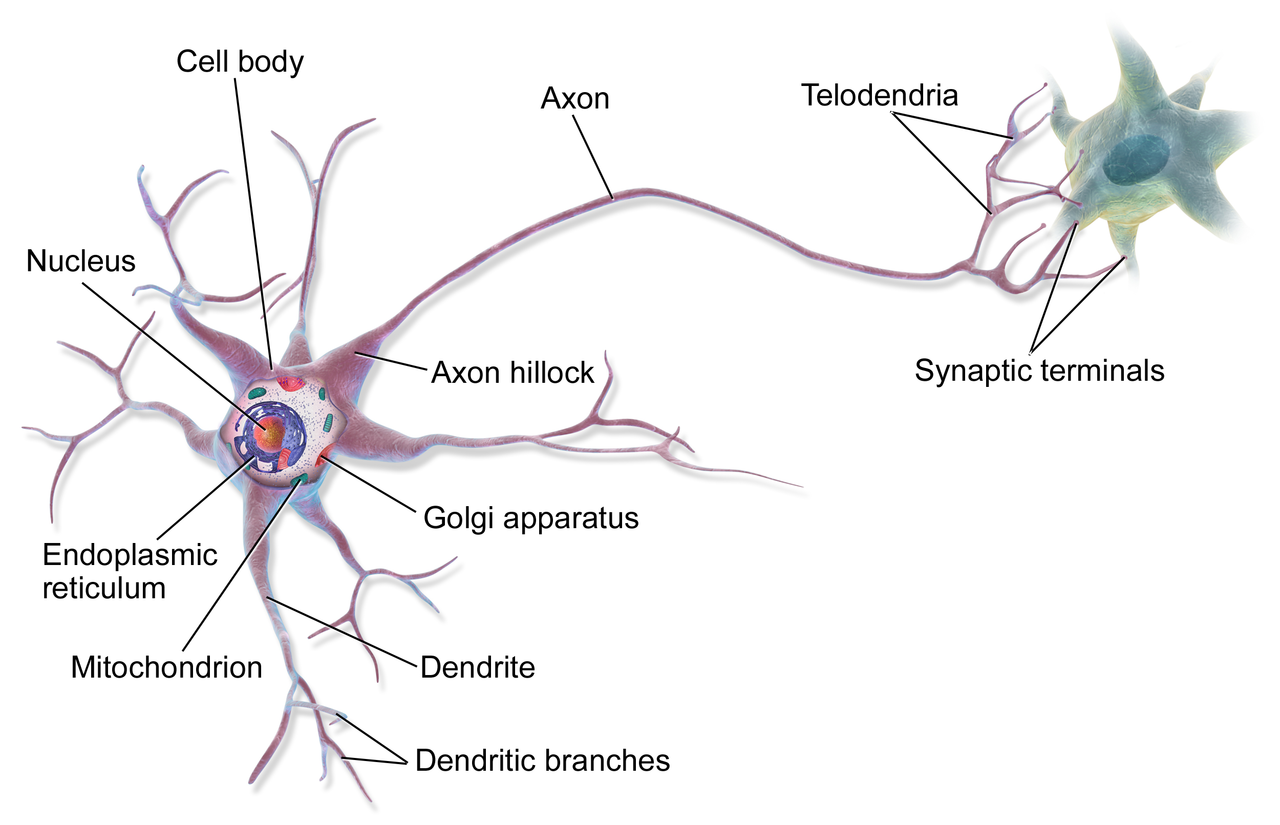
\includegraphics[width=0.9\textwidth]{img/Blausen_0657_MultipolarNeuron.png}
	\end{figure}
	\tiny{Image taken from \url{http://en.wikipedia.org/wiki/File:Blausen_0657_MultipolarNeuron.png}}.
\end{frame}


\begin{frame}
	\frametitle{Neural network: artificial}
	\begin{figure}[!h]
		\centering
		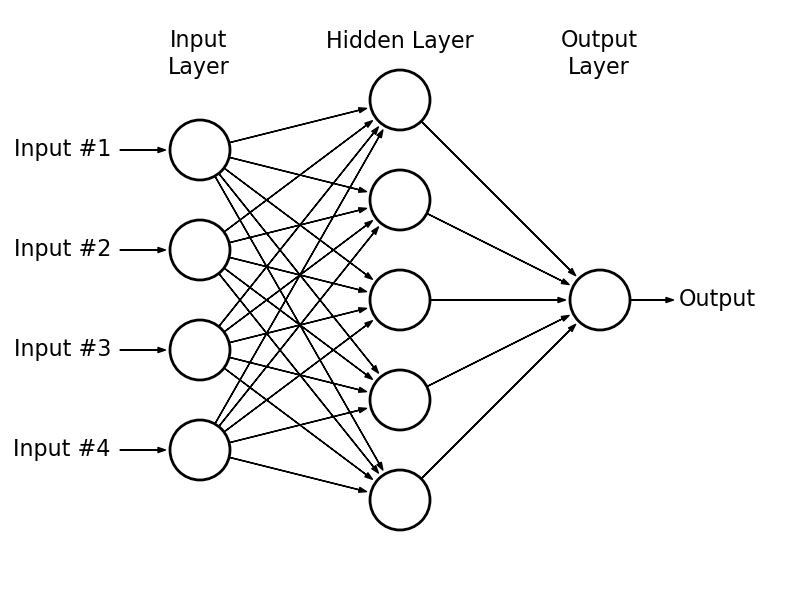
\includegraphics[width=0.9\textwidth]{img/fig_neural_network_1.png}
	\end{figure}
\end{frame}


\end{document}
